\documentclass[10pt,letterpaper]{article}
% Layout of an AIAA conference manuscript, built from standard packages so the draft
% compiles on a stock TeX Live (pdflatex). It follows the AIAA Technical Conference
% paper guidelines: US letter, 1 in margins, 10 pt Times, 24 pt bold title, bold
% indented abstract, centred roman-numbered section headings, lettered subsections,
% "Fig. n" / "Table n" bold captions and bracketed numeric citations.
% For the final submission, paste the body into the official AIAA template
% (new-aiaa.cls, distributed by AIAA through Overleaf); no body text depends on this file.
\usepackage[letterpaper,margin=1in]{geometry}
\usepackage[T1]{fontenc}
\usepackage[utf8]{inputenc}
\usepackage{amsmath,amssymb}
\usepackage{newtxtext,newtxmath}
\usepackage{bm}
\usepackage{graphicx}
\usepackage{xcolor}
\usepackage{booktabs}
\usepackage{array}
\usepackage{longtable}
\usepackage{siunitx}
\usepackage{algorithm}
\usepackage{algpseudocode}
\usepackage{tikz}
\usetikzlibrary{positioning,arrows.meta,fit,backgrounds}
\usepackage[numbers,sort&compress]{natbib}
\usepackage{titlesec}
\usepackage[font={small,bf},labelfont=bf,labelsep=quad]{caption}
\usepackage{enumitem}
\usepackage[hidelinks]{hyperref}

\sisetup{per-mode=symbol, detect-weight=true, group-minimum-digits=5}
\setlength{\parindent}{0.2in}
\setlength{\parskip}{0pt}
\setlist{nosep,leftmargin=0.35in}
\captionsetup[figure]{name=Fig.}
\captionsetup[table]{name=Table,position=top}
\setlength{\bibsep}{2pt}
\renewcommand{\bibfont}{\small}

% Headings: I. Section (centred), A. Subsection (bold), 1. Subsubsection (italic).
\renewcommand{\thesection}{\Roman{section}}
\renewcommand{\thesubsection}{\Alph{subsection}}
\renewcommand{\thesubsubsection}{\arabic{subsubsection}}
\makeatletter
\renewcommand{\p@subsection}{\thesection.}
\renewcommand{\p@subsubsection}{\thesection.\thesubsection.}
\makeatother
\titleformat{\section}{\normalfont\large\bfseries\centering}{\thesection.}{0.5em}{}
\titleformat{\subsection}{\normalfont\normalsize\bfseries}{\thesubsection.}{0.5em}{}
\titleformat{\subsubsection}{\normalfont\normalsize\itshape}{\thesubsubsection.}{0.5em}{}
\titlespacing*{\section}{0pt}{12pt plus 3pt minus 2pt}{6pt}
\titlespacing*{\subsection}{0pt}{9pt plus 2pt minus 2pt}{3pt}
\titlespacing*{\subsubsection}{0pt}{6pt plus 2pt minus 1pt}{2pt}

% Title block and abstract.
\newcommand{\aiaatitle}[1]{\begin{center}\fontsize{24}{28}\selectfont\bfseries #1\par\end{center}\vspace{6pt}}
\newcommand{\aiaaauthor}[1]{\begin{center}\fontsize{16}{19}\selectfont #1\par\end{center}\vspace{-6pt}}
\newcommand{\aiaaaffiliation}[1]{\begin{center}\fontsize{12}{14}\selectfont\itshape #1\par\end{center}\vspace{4pt}}
\newenvironment{aiaaabstract}
  {\begin{list}{}{\setlength{\leftmargin}{0.5in}\setlength{\rightmargin}{0.5in}\setlength{\listparindent}{0.2in}%
   \setlength{\itemindent}{0.2in}\setlength{\parsep}{0pt}}\item\relax\bfseries}
  {\end{list}\vspace{4pt}}
\newenvironment{nomenclature}
  {\section*{Nomenclature}\small\setlength{\LTleft}{0pt}\setlength{\LTpre}{0pt}\setlength{\LTpost}{0pt}%
   \begin{longtable}{@{}l@{\quad=\quad}p{0.78\textwidth}@{}}}
  {\end{longtable}\addtocounter{table}{-1}\normalsize}

% References kept whole.
\newcommand{\refalg}[1]{Algorithm~\ref{#1}}
\newcommand{\refeq}[1]{Eq.~(\ref{#1})}
\newcommand{\refeqs}[2]{Eqs.~(\ref{#1})--(\ref{#2})}
\newcommand{\reffig}[1]{Fig.~\ref{#1}}
\newcommand{\refsec}[1]{Section~\ref{#1}}
\newcommand{\reftab}[1]{Table~\ref{#1}}

% Notation.
\newcommand{\vect}[1]{\bm{#1}}
\newcommand{\mat}[1]{\mathbf{#1}}
\newcommand{\ez}{\hat{\vect{e}}_z}
\newcommand{\wb}{\vect{\omega}}
\newcommand{\mdot}{\dot{m}}
\newcommand{\Ir}{I_r}
\newcommand{\wrot}{\omega_r}
\newcommand{\wmax}{\omega_{\max}}
\newcommand{\uj}{u_j}
\graphicspath{{figures/}{../physics_simulation/figures/}}


\hypersetup{pdftitle={Convex Powered-Descent Guidance with Plant-Derived Constraints for a Jet-Vane Thrust-Vectored Electric Ducted Fan Testbed}, pdfauthor={Tang Zijian (Jacob Tang)}}
\begin{document}

\aiaatitle{Convex Powered-Descent Guidance with Plant-Derived Constraints for a Jet-Vane Thrust-Vectored Electric Ducted Fan Testbed}

{\renewcommand{\thefootnote}{\fnsymbol{footnote}}%
\aiaaauthor{Tang Zijian (Jacob Tang)\footnote{Graduate Student in Data Science, Department of Computer and Information Sciences.}}
\aiaaaffiliation{Minnesota State University, Mankato, Minnesota, 56001}}
\setcounter{footnote}{0}

\begin{aiaaabstract}
A single electric ducted fan steered by four jet vanes is a laboratory analogue of a retro-propulsive stage. Its mass remains constant, the rotor stores angular momentum, and battery voltage limits thrust.
We combine a momentum-based plant with a guidance law that searches over fixed-duration conic programs.
Of 400 dispersed starts, 355 returned hard-terminal plans with a median planning time of \SI{62}{\milli\second}.
The relative node gap between actual and relaxed thrust magnitude exceeded \num{1e-3} in 72 of those plans. A half-space repair reduced the largest relative node gap to \num{6.3e-4} at a median increase of 2\% in planned energy for the 72 cases.
Planned energy rose approximately at hover power over the sampled solved durations. Exact inter-node checks found small residual thrust-floor violations and thrust-direction rates above the nominal \SI{12}{\degree\per\second} scale.
In the reduced-order simulation all 400 runs reached touchdown height, with maximum downward speed \SI{0.206}{\metre\per\second} and pad error \SI{0.333}{\metre}. Eight earlier rigid-body missions recorded maxima of \SI{0.178}{\metre\per\second} pre-contact and \SI{0.146}{\metre} from the pad.
\end{aiaaabstract}

\section{Introduction}

Under the classical losslessness hypotheses, powered-descent guidance with a non-convex thrust magnitude bound admits a second-order cone program (SOCP)~\cite{acikmese2007,acikmese2013lcvx}, and the method has flown on rocket-powered test vehicles~\cite{scharf2017}.
The relaxation has been extended to minimum-landing-error targets~\cite{blackmore2010mle} and, under additional conditions, to state constraints~\cite{harris2014lcvx}; Malyuta et al.\ survey the field~\cite{malyuta2022convex}.
Sub-scale electric vehicles are attractive for exercising such guidance cheaply and repeatedly, and Linsen et al.\ fly optimal control on an electric prototype with gimballed propulsion~\cite{linsen2022}.
Whether the method transfers to such a vehicle depends on two things it does not supply: a plant model that is right about what limits the vehicle, and planning constraints that represent those limits.

The testbed studied here is a \SI{3.1}{\kilogram} vehicle lifted by one \SI{90}{\milli\metre} electric ducted fan and steered by four servo-driven jet vanes in the exhaust.
Its limits are not a rocket's.
The vanes command attitude by redirecting the exhaust. Their torque scales with thrust and depends on the fraction of the jet each vane intercepts.
The rotor stores \SI{0.78}{\newton\metre\second} at hover, and the vanes provide approximately \SI{0.30}{\newton\metre} of net yaw torque. Changing rotor speed exchanges angular momentum with the body, while tilting the rotor axis requires transverse torque.
The vehicle loses no mass, its thrust ceiling follows the battery's loaded voltage, and the cost that matters is electrical energy.
These properties make thrust rate and attitude rate the binding actuator limits.
Neither appears in the classical formulation, and a thrust-rate bound couples successive controls, which lies outside the hypotheses under which the relaxation is known to be lossless~\cite{acikmese2011lcvx,harris2014lcvx}.
Ducted-fan models include momentum drag at the intake~\cite{johnson2006ducted}. Here the rotor and finite vane authority also enter the planning limits.

The paper makes four contributions.
\begin{enumerate}
\item A momentum-based jet-vane model with a closed-form small-angle authority and an isolated torque-free gyrostat conservation check.
\item A constant-mass guidance formulation with thrust, slew and sink constraints and explicit authority reserves.
\item Measurements of relaxation gaps at nodes, thrust magnitude and direction rate between nodes, and energy over a grid of candidate durations.
\item A dispersed closed-loop assessment with matched perturbations of vane authority, rotor inertia, center of mass and planning delay.
\end{enumerate}
The work is a simulation study; no hardware has flown.

\section{Approach}

\textit{Plant model.}
The vehicle is simulated in a GPU rigid-body engine that integrates only the articulated bodies, joint drives and contact; every other effect is a batched force model applied as an external wrench.
A control-volume jet-vane model shares the jet's mass flow among four streamtubes and conserves angular momentum.
In an unswirled axial jet it reduces to the closed-form side force
\begin{equation}
F_{\perp} = \frac{T}{4}\left(\tau_t - \delta_D\right)\sin\alpha\cos\alpha ,
\end{equation}
in which the uncertain lift slope nearly drops out ($\tau_t = 0.9995$ at the modeled loading); the earlier independent-airfoil model gave 8.5 times the modeled small-angle authority.
A current-limited motor is coupled to a Thevenin battery circuit with an energy cap, and the rotor's spool, swirl and gyroscopic reactions are applied at full strength.
At hover rotor speed, intake momentum drag exceeds modeled crossflow drag below \SI{12.3}{\metre\per\second}. Together with the duct-flow Coriolis reaction, it recovers the classical jet-damping moment.
In the isolated torque-free test with constant hover rotor speed and zero axial body spin, explicit Euler integration at \SI{120}{\hertz} amplifies transverse body kinetic energy 57-fold in two seconds. The coupled implicit-midpoint and Cayley updates conserve body kinetic energy and world angular momentum to round-off.
At a transverse body rate of \SI{1}{\radian\per\second}, the effective roll and pitch damping coefficient is $1/131$ of the earlier tuned value. The earlier attitude law has an unstable mode on the corrected plant at hover.

\begin{figure}[!t]
\centering
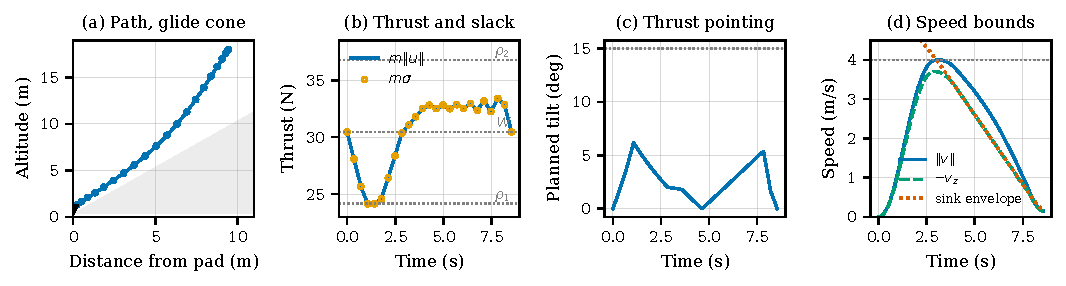
\includegraphics[width=\textwidth]{convex_plan.pdf}
\caption{Reference plan from $(8, 5, 18)$ m at rest. Panels show the path and glide cone, thrust and slack at the nodes, planned tilt, and the speed and sink-rate bounds.}
\label{fig:plan}
\end{figure}

\textit{Guidance.}
The planner models a constant-mass point with thrust acceleration $\vect{u}$. Each fixed-duration relaxation uses second-order cones for trajectory constraints and native power cones for the quasi-steady energy objective.
Constraints include a relaxed thrust annulus, pointing cone, rates on the full and horizontal thrust vectors, glide slope, speed and sink rate. The sink envelope uses 35\% of the upright planned braking acceleration and includes a decaying allowance for fast entries.
The thrust is linear between nodes, beginning from a projected measured thrust or the preceding plan's reference thrust.
The bounds are derived at every re-plan from the plant and the measured bus voltage $V$ (with nominal reference $V_{\text{ref}} = \SI{29.6}{\volt}$ and vane effort limit $\bar\alpha = \SI{0.245}{\radian}$, reserving the $\SI{0.017}{\radian}$ servo deadband out of the $\SI{0.262}{\radian}$ travel):
\begin{equation}
\rho_2 = \max\!\left(1.01W,\,W+\tfrac12(T_{\text{av}}(V)-W)\right), \qquad
\Ir\wmax\frac{V}{V_{\text{ref}}}\,\dot d \le 0.4\,\min\!\left(K_\psi f_h^2\bar\alpha,\, \tau_\psi\right), \qquad
\omega_t \le 0.4\,\frac{K f_h^2\bar\alpha}{\Ir\wmax f_h} ,
\end{equation}
The numerical minimum on the ceiling matters below the sampled voltage range. At \SI{24.4}{\volt} the model can supply only \SI{29.26}{\newton} against \SI{30.45}{\newton} of weight, while the planner permits \SI{30.75}{\newton}. The 0.4 factors allocate hover torque to commanded slew.
The planner selects a duration by a line search over fixed-duration problems solved in parallel with an interior-point conic solver~\cite{goulart2024clarabel}.
Every plan reports its convexification gap $\epsilon = \max_k\big[(\sigma_k - \|\vect{u}_k\|)/\sigma_k\big]$.
When the gap exceeds \num{e-3} the gapped nodes receive a convex half-space thrust floor along their solved thrust direction and the problem is solved once more.
\reffig{fig:plan} shows a representative plan, which descends on its speed bound and brakes along the sink-rate envelope.
A scheduled full-state linear-quadratic regulator that feeds back both actuator states realizes the plan on the vanes.

\section{Results to Date}

All planner and plant-model results are computed by scripts that import the production code. Closed-loop results are of two kinds: a dispersed campaign that flies the production flight computer on a reduced-order replica of the plant, and recorded runs in the rigid-body engine.

\textit{Planner over dispersed starts.}
Four hundred starts were drawn with offsets up to \SI{25}{\metre}, altitudes of 5--\SI{40}{\metre}, horizontal speeds up to \SI{3}{\metre\per\second}, vertical speeds from \SI{-3}{} to \SI{+1}{\metre\per\second}, and bus voltages of 26--\SI{33}{\volt} (\reftab{tab:mc}, \reffig{fig:mc}).
The search returned 355 hard-terminal plans and 45 soft-terminal fallbacks. A finer duration sweep found a hard-terminal solution for fallback case 336 at \SI{17.75}{\second}.
Among the 355 hard-terminal results, planning took a median of \SI{62}{\milli\second} and at most \SI{117}{\milli\second} on the laptop processor.

\textit{Losslessness.}
Before repair, 72 of the 355 hard-terminal plans had node gaps above \num{e-3}, up to 3.4\%.
Re-solving those cases at the same durations with only the full-vector rate bound removed left 47 above tolerance.
Repair reduced the maximum node gap to \num{6.3e-4}. Between nodes, 121 of the 355 plans dipped below the thrust floor by more than \SI{e-5}{\newton} (worst \SI{0.125}{\newton}), and 131 exceeded the horizontal-rate proxy's nominal \SI{12.01}{\degree\per\second} when measured on the unit thrust direction (peak \SI{16.35}{\degree\per\second}).

\textit{Structure of the free-final-time problem.}
With the guard disabled, 53 of 60 starts had solutions on the \SI{0.5}{\second} grid. Across contiguous solved samples, cost was non-decreasing and the fitted slopes were 0.577--\SI{0.579}{\watt\hour\per\second}, close to hover power.
For the reference start the normal search returned \SI{8.544}{\second} and \SI{4.9668}{\watt\hour}. A finer fixed-duration check yielded \SI{8.45}{\second} and \SI{4.9201}{\watt\hour}. The sampled durations establish neither the exact feasibility boundary nor a global optimum.

\textit{Dispersed closed loop.}
The unmodified flight computer was flown from the same 400 starts, each with a steady wind of up to \SI{4}{\metre\per\second}, on a replica with the rotor's gyroscopic and spool reactions, vane torques and their side force, the servo deadband and joint lag, the current-limited motor, and intake and body drag; the replica has no contact model and the controller reads the true state.
All 400 runs passed the downward-speed and pad-error criteria at the first body-origin touchdown-height crossing, including the 46 that tracked a soft-terminal plan. The maximum total body speed there was \SI{0.228}{\metre\per\second}.
All 100 matched cases also passed with a fixed \SI{0.4}{\second} re-plan delay, a 20\% increase in rotor inertia, or a \SI{5}{\milli\metre} center-of-mass offset, tested separately.
With vanes 30\% weaker than modeled, 93 of 100 runs passed, two crossed off the pad and five timed out. This perturbation caused the largest loss of completions among those tested.
The earlier proportional-derivative attitude law is linearly unstable on this plant above 67\% rotor speed, whereas the regulator's slowest mode decays at 1.9--\SI{2.0}{\per\second} there (1.6--\SI{2.0}{\per\second} across 30--100\% rotor speed).
On the same starts, median roll and pitch rate RMS increased from 2.8 to \SI{12.2}{\degree\per\second} with the earlier law, consistent with the bounded oscillations observed in simulation.

\textit{Recorded missions.}
Eight recorded missions on the momentum-vane plant---direct descents from 3 to \SI{50}{\metre}, an offset start with crosswind, waypoint routes with hovers, the legacy six-cell pack, and a combined wind, sensor-noise and mass-offset case---landed with impacts of 0.136--\SI{0.178}{\metre\per\second} and pad errors of 0.004--\SI{0.146}{\metre} against limits of \SI{0.25}{\metre\per\second} and \SI{0.5}{\metre}.
These eight runs preceded the sink-rate envelope, emergency braking, corrected intake station, duct Coriolis term and node-gap guard. The project hosts a read-only replay at \url{https://triaggent.com/portfolio/mission-control/}.

\begin{table}[t]
\caption{Planner outcome over 400 dispersed starts}
\label{tab:mc}
\centering
\small
\begin{tabular}{lcc}
\toprule
 & Relaxation as solved & With gap guard \\
\midrule
Hard-terminal / soft-terminal / no plan & 355 / 45 / 0 & 355 / 45 / 0 \\
Hard-terminal plans with gap above \num{e-3} & 72 (20\%) & 0 \\
Largest gap & \num{3.4e-2} & \num{6.3e-4} \\
Energy change on the gapped plans, median / maximum & --- & $+2.0\%$ / $+10.3\%$ \\
Hard-terminal wall time, median / maximum & 61 / \SI{95}{\milli\second} & 62 / \SI{117}{\milli\second} \\
\bottomrule
\end{tabular}
\end{table}

\begin{figure}[t]
\centering
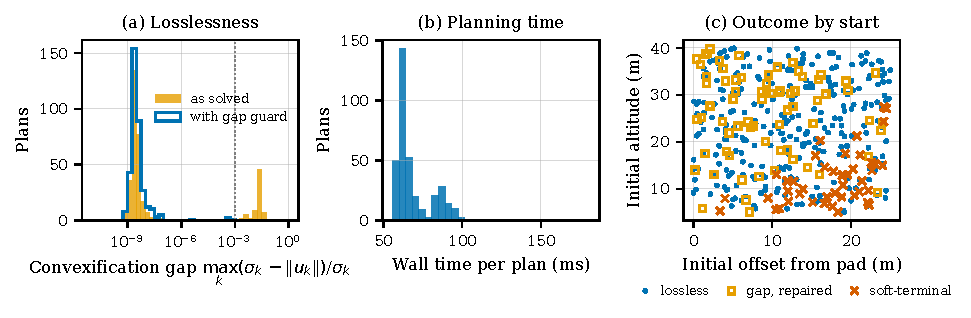
\includegraphics[width=0.82\textwidth]{planner_mc.pdf}
\caption{Planner outcomes for 400 dispersed starts. The gap distributions and timing histogram in (a) and (b) cover the 355 hard-terminal plans. Panel (c) includes all starts.}
\label{fig:mc}
\end{figure}


\section{Expected Final Results}

The full paper gives the plant model with its verification (unit tests, offline runs of the production code, and a recorded open-loop audit in which nutation frequency, precession rate and momentum exchange match first-principles predictions to within about 5\%), the complete guidance formulation and its derivation from the plant, the flight controller, the planner studies summarized above with a discretization study, and the closed-loop missions.
It also states the limits of the evidence: several parameters are planning estimates (with jet-speed convention, streamtube share and rotor inertia identified to measure first), the planner omits aerodynamics, the dispersed closed-loop replica omits contact and sensing, the latest plant terms and gap guard await rigid-body re-flight, and no hardware has flown.

The next phase of the work, for the final manuscript, has two parts.
\begin{enumerate}
\item \textit{Geometric integrators and full-simulator verification.} Comparing the explicit, rotor-only midpoint and coupled midpoint--Cayley schemes against other structure-preserving gyrostat integrators across step sizes and spin rates, and re-flying the recorded and dispersed campaigns in the full simulator with all latest terms and the gap guard.
\item \textit{Bench identification and hardware transfer.} Static thrust-stand measurement of $T(\wrot, V)$, exhaust speed, independently measured rotor inertia $\Ir$, coast-down drag, loaded servo response, and vane side force and drag, followed by closed-loop evaluation on the identified plant and, as bring-up permits, tethered and free-flight tests.
\end{enumerate}

\setlength{\bibsep}{0pt}
\begin{thebibliography}{99}

\bibitem{acikmese2007}
A\c{c}{\i}kme\c{s}e, B., and Ploen, S. R., ``Convex Programming Approach to Powered Descent Guidance for Mars Landing,'' \textit{Journal of Guidance, Control, and Dynamics}, Vol.~30, No.~5, 2007, pp.~1353--1366.

\bibitem{acikmese2013lcvx}
A\c{c}{\i}kme\c{s}e, B., Carson, J. M., and Blackmore, L., ``Lossless Convexification of Nonconvex Control Bound and Pointing Constraints of the Soft Landing Optimal Control Problem,'' \textit{IEEE Transactions on Control Systems Technology}, Vol.~21, No.~6, 2013, pp.~2104--2113.

\bibitem{scharf2017}
Scharf, D. P., A\c{c}{\i}kme\c{s}e, B., Dueri, D., Benito, J., and Casoliva, J., ``Implementation and Experimental Demonstration of Onboard Powered-Descent Guidance,'' \textit{Journal of Guidance, Control, and Dynamics}, Vol.~40, No.~2, 2017, pp.~213--229.

\bibitem{blackmore2010mle}
Blackmore, L., A\c{c}{\i}kme\c{s}e, B., and Scharf, D. P., ``Minimum-Landing-Error Powered-Descent Guidance for Mars Landing Using Convex Optimization,'' \textit{Journal of Guidance, Control, and Dynamics}, Vol.~33, No.~4, 2010, pp.~1161--1171.

\bibitem{harris2014lcvx}
Harris, M. W., and A\c{c}{\i}kme\c{s}e, B., ``Lossless Convexification of Non-Convex Optimal Control Problems for State Constrained Linear Systems,'' \textit{Automatica}, Vol.~50, No.~9, 2014, pp.~2304--2311.

\bibitem{malyuta2022convex}
Malyuta, D., Reynolds, T. P., Szmuk, M., Lew, T., Bonalli, R., Pavone, M., and A\c{c}{\i}kme\c{s}e, B., ``Convex Optimization for Trajectory Generation: A Tutorial on Generating Dynamically Feasible Trajectories Reliably and Efficiently,'' \textit{IEEE Control Systems Magazine}, Vol.~42, No.~5, 2022, pp.~40--113.

\bibitem{linsen2022}
Linsen, R., Listov, P., de Lajarte, A., Schwan, R., and Jones, C. N., ``Optimal Thrust Vector Control of an Electric Small-Scale Rocket Prototype,'' \textit{Proceedings of the IEEE International Conference on Robotics and Automation (ICRA)}, 2022, pp.~1996--2002.

\bibitem{acikmese2011lcvx}
A\c{c}{\i}kme\c{s}e, B., and Blackmore, L., ``Lossless Convexification of a Class of Optimal Control Problems with Non-Convex Control Constraints,'' \textit{Automatica}, Vol.~47, No.~2, 2011, pp.~341--347.

\bibitem{johnson2006ducted}
Johnson, E. N., and Turbe, M. A., ``Modeling, Control, and Flight Testing of a Small Ducted-Fan Aircraft,'' \textit{Journal of Guidance, Control, and Dynamics}, Vol.~29, No.~4, 2006, pp.~769--779.

\bibitem{goulart2024clarabel}
Goulart, P. J., and Chen, Y., ``Clarabel: An Interior-Point Solver for Conic Programs with Quadratic Objectives,'' \textit{Mathematical Programming Computation}, Vol.~18, 2026, pp.~1279--1361.

\end{thebibliography}

\end{document}
